\section{Auswertung}
\label{sec:Auswertung}
Die Messung wird nach \autoref{sec:Durchführung} durchgeführt und die Temperatur- und Druckverläufe, sowie die Leistungsaufnahme des Kompressors
werden in \autoref{tab:Tab1} in Abhängigkeit von der Zeit dargestellt.
Hierbei werden die Werte direkt in SI-Einheiten umgerechnet und zu den Drücken, wie in der Versuchsanleitung \cite{V206} vorgegeben, 
$\qty{1}{bar}$ addiert.
\begin{table}[H]
	\centering
	\caption{Messwerte der Wärmepumpe.}
	\label{tab:Tab1}
  \sisetup{table-format=3.2}
	\begin{tabular}{S[table-format=4.0] S S S[table-format=1.1] S[table-format=2.1] S[table-format=3.0]}
		\toprule
      {$t \mathbin{/} \si{\second}$}&{$T_1 \mathbin{/} \si{\kelvin}$}&{$T_2 \mathbin{/} \si{\kelvin}$}&{$p_a \cdot 10^{-5} \mathbin{/} \si{\pascal}$}&{$p_b \cdot 10^{-5} \mathbin{/} \si{\pascal}$} &
      {$N \mathbin{/} \si{\watt}$}\\
    \midrule
      0 & 294,15 & 293,85 & 4,8 & 4,5 & 0\\
      60 & 294,85 & 293,75 & 4,0 & 6,0 & 115\\
      120 & 296,05 & 292,65 & 4,2 & 6,5 & 120\\
      180 & 297,55 & 291,15 & 4,4 & 6,8 & 122\\
      240 & 299,05 & 289,75 & 4,4 & 7,0 & 125\\
      300 & 300,55 & 288,55 & 4,4 & 7,1 & 125\\
      360 & 302,05 & 287,45 & 4,2 & 7,5 & 122\\
      420 & 303,45 & 286,45 & 4,0 & 7,9 & 122\\
      480 & 304,85 & 285,35 & 4,0 & 8,0 & 122\\
      540 & 306,15 & 284,35 & 3,8 & 8,3 & 122\\
      600 & 307,35 & 283,45 & 3,7 & 8,8 & 122\\
      660 & 308,45 & 282,55 & 3,6 & 9,0 & 125\\
      720 & 309,65 & 281,65 & 3,5 & 9,1 & 125\\
      780 & 310,65 & 280,75 & 3,4 & 9,5 & 125\\
      840 & 311,65 & 279,85 & 3,4 & 9,7 & 125\\
      900 & 312,65 & 279,05 & 3,2 & 10,0 & 115\\
      960 & 314,45 & 278,15 & 3,2 & 10,2 & 115\\
      1020 & 314,45 & 277,35 & 3,2 & 10,2 & 115\\
      1080 & 315,25 & 276,75 & 3,0 & 10,5 & 115\\
      1140 & 316,05 & 276,05 & 3,0 & 11,0 & 115\\
      1200 & 316,75 & 275,35 & 3,0 & 11,0 & 115\\
      1260 & 317,55 & 274,75 & 2,9 & 11,2 & 115\\
      1320 & 318,95 & 274,05 & 2,8 & 11,5 & 115\\
      1380 & 318,95 & 273,45 & 2,8 & 11,5 & 115\\
      1440 & 319,55 & 272,95 & 2,7 & 11,8 & 115\\
      1500 & 320,15 & 272,45 & 2,7 & 12,0 & 115\\
      1560 & 320,75 & 271,85 & 2,7 & 12,0 & 115\\
      1620 & 321,35 & 271,35 & 2,6 & 12,1 & 110\\
      1680 & 321,95 & 270,75 & 2,6 & 12,2 & 110\\
      1740 & 322,45 & 270,35 & 2,6 & 12,3 & 110\\
      1800 & 322,95 & 269,85 & 2,5 & 12,6 & 110\\
      1860 & 323,55 & 269,85 & 2,5 & 13,0 & 110\\
    \bottomrule
  \end{tabular}
\end{table}

Aus den Werten in \autoref{tab:Tab1} für die Temperaturen $T_1$ und $T_2$ wird ein Plot erstellt, siehe \autoref{fig:plot1}.
Hier werden die Temperaturverläufe in Abhängigkeit von der Zeit aufgetragen.

\begin{figure}
  \centering
  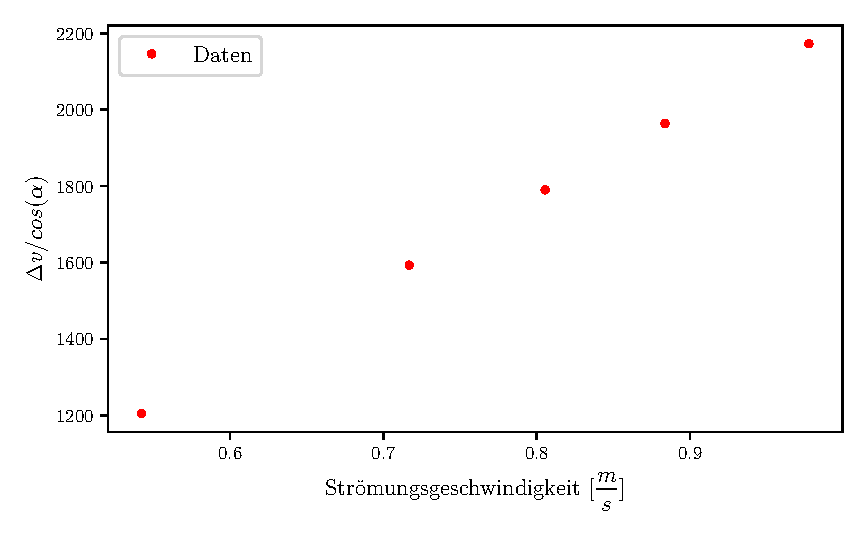
\includegraphics{plot1.pdf}
  \caption{Temperaturverläufe von $T_1$ und $T_2$.}
  \label{fig:plot1}
\end{figure}

Außerdem wird nach der Formel
\begin{align*}
  T(t)=at^2+bt+c
\end{align*}
jeweils eine Ausgleichskurve für $T_1$ und $T_2$ erstellt.
Die Parameter werden mithilfe von Python bestimmt und lauten für die Ausgleichskurve von $T_1$
\begin{align*}
  a&= (-5,5677 \pm 0,1998) \cdot 10^{-6} \si{\kelvin\per\second\squared}\\
  b&= (0,0264 \pm 0,0004) \si{\kelvin\per\second}\\
  c&= (293,37 \pm 0,15) \si{\kelvin},
\end{align*}
und für die Ausgleichskurve von $T_2$
\begin{align*}
  a&= (4,0330 \pm 0,1331) \cdot 10^{-6} \si{\kelvin\per\second\squared}\\
  b&= (-0,0209 \pm 0,0003) \si{\kelvin\per\second}\\
  c&= (294,56 \pm 0,10) \si{\kelvin}.
\end{align*}


Aus den in \autoref{fig:plot1} dargestellten Funktionen werden nun die Differenzenquotienten $\frac{dT_1}{dt}$ und $\frac{dT_2}{dt}$ zu vier gewählten
Zeitpunkten bestimmt. Die gewählten Zeitpunkte sind\\ $t_1=\qty{420}{\second},t_2=\qty{840}{\second}, t_3=\qty{1260}{\second}$ und $t_4=\qty{1680}{\second}$.
Im Folgenden werden alle zu bestimmenden Größen jeweils zu diesen Zeitpunkten berechnet.
Die Differenzenquotienten werden nach
\begin{align*}
  \frac{dT}{dt}&= 2at+b
  \intertext{berechnet, wobei der Fehler durch}
  \Delta \frac{dT}{dt}&= \sqrt{(2t\cdot \Delta a)^2+(\Delta b)^2}
\end{align*}
bestimmt wird. In \autoref{tab:Tab2} sind die Differenzenquotienten $\frac{dT_1}{dt}$ und $\frac{dT_2}{dt}$ und ihre Fehler zu den vier gewählten
Zeitpunkten aufgelistet.
\begin{table}[H]
	\centering
	\caption{Differenzenquotienten von Temperaturen $T_1$ und $T_2$ zu vier gewählten Zeitpunkten.}
	\label{tab:Tab2}
  \sisetup{table-format=1.4}
	\begin{tabular}{S[table-format=4.0] S[table-format=3.2] S@{${}\pm{}$}S S[table-format=3.2] S[table-format=3.4]@{${}\pm{}$}S}
		\toprule
      {$t \mathbin{/} \si{\second}$}&{$T_1 \mathbin{/} \si{\kelvin}$}&\multicolumn{2}{c}{$\frac{dT_1}{dt} \mathbin{/} \si{\kelvin\per\second}$}&{$T_2 \mathbin{/} \si{\kelvin}$}&\multicolumn{2}{c}{$\frac{dT_2}{dt}\mathbin{/} \si{\kelvin\per\second}$}\\
    \midrule
    420  & 303,45 & 0,0217 & 0,0004 & 286,45 & -0,0175 & 0,0003 \\
    840  & 311,65 & 0,0170 & 0,0005 & 279,85 & -0,0141 & 0,0003 \\
    1260 & 317,55 & 0,0124 & 0,0006 & 274,75 & -0,0107 & 0,0004 \\
    1680 & 321,95 & 0,0077 & 0,0008 & 270,75 & -0,0073 & 0,0005 \\
    \bottomrule
  \end{tabular}
\end{table}	

Im nächsten Schritt sollen die ideale und die reale Güteziffer der Wärmepumpe nach Gleichungen \ref{eqn:Güteziffer_ideal} und \ref{eqn:Güteziffer}
bestimmt werden. N wird dafür gemittelt aus \autoref{tab:Tab1} zu\\ $\bar{N}= (114 \pm 4) \si{\watt}$.
Die Wärmekapazität des Wassers beträgt $c_w = \qty{4182}{\joule\per\kilo\gram\per\kelvin}$ \cite[381]{PhyPrak}, die Masse des Wassers im Reservoir
beträgt $m_1= \qty{3}{\kilo\gram}$. Somit wird $m_1c_w$ berechnet zu $m_1c_w= \qty{12546}{\joule\per\kelvin}$. Die Wärmekapazität des Eimers und der 
Kupferschlange beläuft sich auf $m_kc_k=\qty{750}{\joule\per\kelvin}$.
Mit den Werten aus \autoref{tab:Tab2} werden nun die Güteziffern bestimmt und in \autoref{tab:Tab3} dargestellt.
Der Fehler der realen Güteziffer wird nach der Gaußschen Fehlerfortpflanzung durch
\begin{align*}
  \Delta \nu_{real}&= \sqrt{\Bigl(\frac{m_1 c_w + m_k c_k}{\bar{N}}\Delta\frac{dT_1}{dt}\Bigr)^2+\Bigl(-(m_1 c_w + m_k c_k)\frac{dT_1}{dt}\frac{1}{\bar{N}^2}\Delta \bar{N}\Bigr)^2}
\end{align*}
bestimmt.
\begin{table}[H]
	\centering
	\caption{Reale und ideale Güteziffer zu vier gewählten Zeitpunkten.}
	\label{tab:Tab3}
  \sisetup{table-format=1.2}
	\begin{tabular}{S[table-format=4.0] S@{${}\pm{}$}l S[table-format=2.2] S[table-format=2.1]}
		\toprule
      {$t \mathbin{/} \si{\second}$}&\multicolumn{2}{c}{reale Güteziffer $\nu_{real}$}&{ideale Güteziffer $\nu_{ideal}$}&{Abweichung $\mathbin{/} \si{\percent}$}\\
    \midrule
      420  & 2,53 & 0,10 & 17,85 & 85,0 \\
      840  & 1,99 & 0,09 &  9,80 & 79,7 \\
      1260 & 1,44 & 0,09 &  7,42 & 80,6 \\
      1680 & 0,90 & 0,09 &  6,29 & 85,8 \\
    \bottomrule
  \end{tabular}
\end{table}

Die Abweichung der realen von der idealen Güteziffer wird durch die Formel
\begin{align*}
  abw = 100\cdot \Bigl(\frac{\nu_{real}-\nu_{ideal}}{\nu_{ideal}}\Bigr)
\end{align*}
bestimmt.

Um den Massendurchsatz $\frac{\Delta m}{\Delta t}$ nach \autoref{eqn:Massendurchsatz} zu bestimmen wird zuerst ein Plot des logarithmierten
Drucks $\frac{p_b}{p_0}$ in Abhängigkeit von $\frac{1}{T_1}$ erstellt, woraus die Verdampfungswärme $L$ durch
\begin{align}
  L&= -a R\label{eqn:Lar}
\end{align}
bestimmt wird. Die universelle Gaskonstante lautet $R=\qty{8.31446261815324}{\joule\per\mol\per\kelvin}$ und $p_0= \qty{100000}{\pascal}$.

\begin{figure}
  \centering
  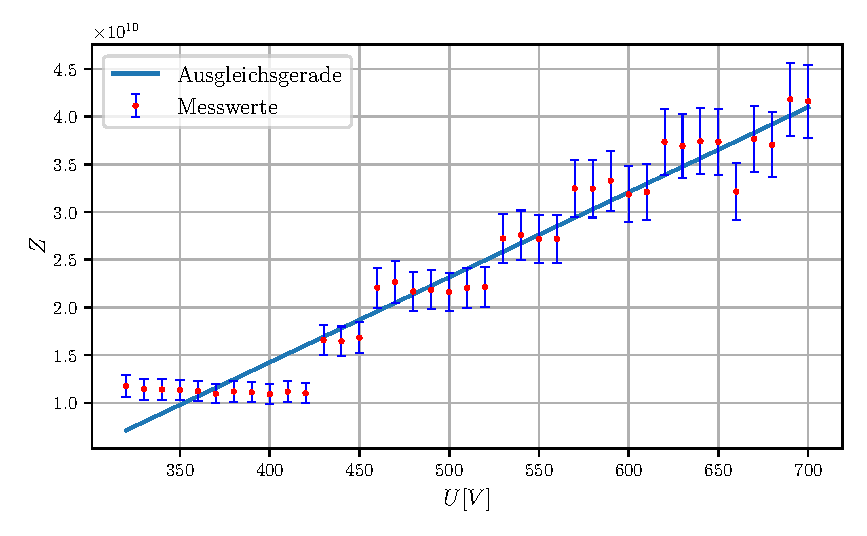
\includegraphics{plot2.pdf}
  \caption{Dampfdruckkurve von Dichlordifluormethan zur Bestimmung der Verdampfungswärme $L$.}
  \label{fig:plot2}
\end{figure}
Die Ausgleichsgerade wird nach $y= a\cdot x+b$ mithilfe von Python bestimmt, daher lauten die Parameter
\begin{align*}
  a&= (-2621.10 \pm 97.45) \si{\kelvin}\\
  b&= (10.67 \pm 0.31)\\
  \intertext{und L kann nach \autoref{eqn:Lar} bestimmt werden zu}
  L&= (21793.07 \pm 810.28) \si{\joule\per\mol}.
\end{align*}

Der berechnete Massendurchsatz wird in \autoref{tab:Tab4} aufgetragen und zur besseren Darstellung in SI-Einheiten mit der molaren Masse von Dichlordifluormethan
$M= \qty{120.9}{\gram\per\mol}$ multipliziert.
Der Fehler des Massendurchsatzes wird durch die Gaußsche Fehlerfortpflanzung nach
\begin{align*}
  \Delta \frac{\Delta m}{\Delta t}&= \sqrt{\Bigl(\frac{m_2 c_w + m_k c_k}{L}\Delta\frac{dT_2}{dt}\Bigr)^2+\Bigl(-(m_2 c_w + m_k c_k)\frac{dT_2}{dt}\frac{1}{L^2}\Delta L\Bigr)^2}
\end{align*}
berechnet.
\begin{table}[H]
	\centering
	\caption{Massendurchsatz zu vier gewählten Zeitpunkten.}
	\label{tab:Tab4}
  \sisetup{table-format=1.4}
	\begin{tabular}{S[table-format=4.0] S[table-format=3.4]@{${}\pm{}$}S[table-format=1.4] S[table-format=3.2]@{${}\pm{}$} S[table-format=1.2]}
		\toprule
      {$t \mathbin{/} \si{\second}$}&\multicolumn{2}{c}{$\frac{dm}{dt} \mathbin{/} \si{\mol\per\second}$}&\multicolumn{2}{c}{$\frac{dm}{dt} \mathbin{/} \si{\gram\per\second}$}\\
    \midrule
      420  & -0,0107 & 0,0004 & -1,29 & 0,05\\
      840  & -0,0086 & 0,0004 & -1,04 & 0,05\\
      1260 & -0,0065 & 0,0004 & -0,79 & 0,04\\
      1680 & -0,0045 & 0,0004 & -0,54 & 0,04\\
    \bottomrule
  \end{tabular}
\end{table}
In \autoref{tab:Tab5} ist die Dichte des Transportgases Dichlordifluormethan, sowie die mechanische Leistung des Kompressors für die vier 
gewählten Zeitpunkte dargestellt.
Die Dichte wird nach der Formel
\begin{align*}
  \rho&= \frac{\rho_0\cdot T_0 \cdot p_a}{T_2 \cdot p_0}
\end{align*} 
berechnet. Hier ist $p_0= \qty{100000}{\pascal}$, $T_0= \qty{273.15}{\kelvin}$ und $\rho_0= \qty{5.51}{\kilo\gram\per\cubic\meter}$.
Mithilfe von \autoref{eqn:Kompressorleistung} und den zuvor berechneten Werten wird somit die mechanische Kompressorleistung bestimmt.
$\kappa$ entspricht für Dichlordifluormethan $\kappa=\qty{1.14}{\watt\per\meter\per\kelvin}$.
Der Fehler der mechanischen Kompressorleistung berechnet sich hierbei durch
\begin{align*}
 \Delta N_{mech} = \sqrt{\Bigl( \frac{1}{\kappa - 1} \Bigl(p_b \sqrt[\kappa]{\frac{p_a}{p_b}}-p_a \Bigr) \frac{1}{\rho} \Delta \frac{\Delta m}{\Delta t}\Bigr)^2}.
\end{align*}
\begin{table}[H]
	\centering
	\caption{Dichte und mechanische Leistung des Kompressors zu vier gewählten Zeitpunkten.}
	\label{tab:Tab5}
  \sisetup{table-format=2.1}
	\begin{tabular}{S[table-format=4.0] S[table-format=2.2] S@{${}\pm{}$} S[table-format=1.1]}
		\toprule
      {$t \mathbin{/} \si{\second}$}&{$\rho \mathbin{/} \si{\kilo\gram\per\cubic\meter}$}&\multicolumn{2}{c}{$N_{mech} \mathbin{/} \si{\watt}$}\\
    \midrule
      420  & 21,02 & 15,3 & 0,6\\
      840  & 18,29 & 19,0 & 0,8\\
      1260 & 15,89 & 18,6 & 1,0\\
      1680 & 14,45 & 14,5 & 1,2\\
      \bottomrule
    \end{tabular}
  \end{table}





